%************************************************
\chapter{Objectives and Methodology}\label{ch:objandmeth}
%************************************************

%TODO resumir organización del capítulos

\section{Project description}


\section{Working methodology}


\section{Development environment}


\subsection{Hardware}

To test our design in a realistic but easy  to work with deployment, we used as the \ac{IoT} device an Onion Omega2 development board, and as the delegation server a Raspberry Pi 3.


\paragraph{Onion Omega2:}\marginpar{
	\vskip0pt
	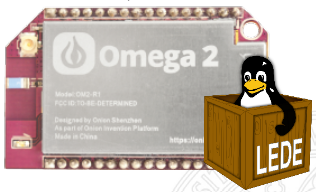
\includegraphics[width=\linewidth]{gfx/Omega2}
	
	Onion Omega2
} A device that falls inside the second category of IoT, powerful enough to run a familiar Linux environment, where we can develop and debug the first \acp{PoC} without troubling ourselves with non-related to the project problems.

Nonetheless, the Omega2 needs fine tunning to start operating, and basic knowledge of electronics is vital to make it work. The two main things to begin with Omega2 are:
\begin{itemize}
	\item A reliable 3.3V with a maximum of 800mA power supply (a USB with a step-down circuit works fine), with quality soldering and wires to avoid unwanted resistances.
	\item A Serial to USB adapter wired to the TX and RX UART pins to use the Serial Terminal, in case WiFi doesn't work and no SSH is available, and because the connection is more reliable in case of wireless interferences.
\end{itemize}


\begin{table}[h]
	\myfloatalign
	\begin{tabularx}{0.75\textwidth}{ll} \toprule
		MCU & Mediatek MT688 \citep{MT7688} \\
		CPU & MIPS32 24KEc 580MHz \\
		RAM & 64MB \\
		Storage & 16MB \\
		Firmware & LEDE (OpenWRT fork distro) \\
		Connectivity & Wifi b/g/n \\
		Power & 3.3V 300mA \\
		\bottomrule
	\end{tabularx}
	\caption[Onion Omega 2 Specifications]{Onion Omega2 Specifications.}
	\label{tab:Omega2Specs}
\end{table}




\paragraph{Raspberry Pi 3:}\marginpar{
	\vskip0pt
	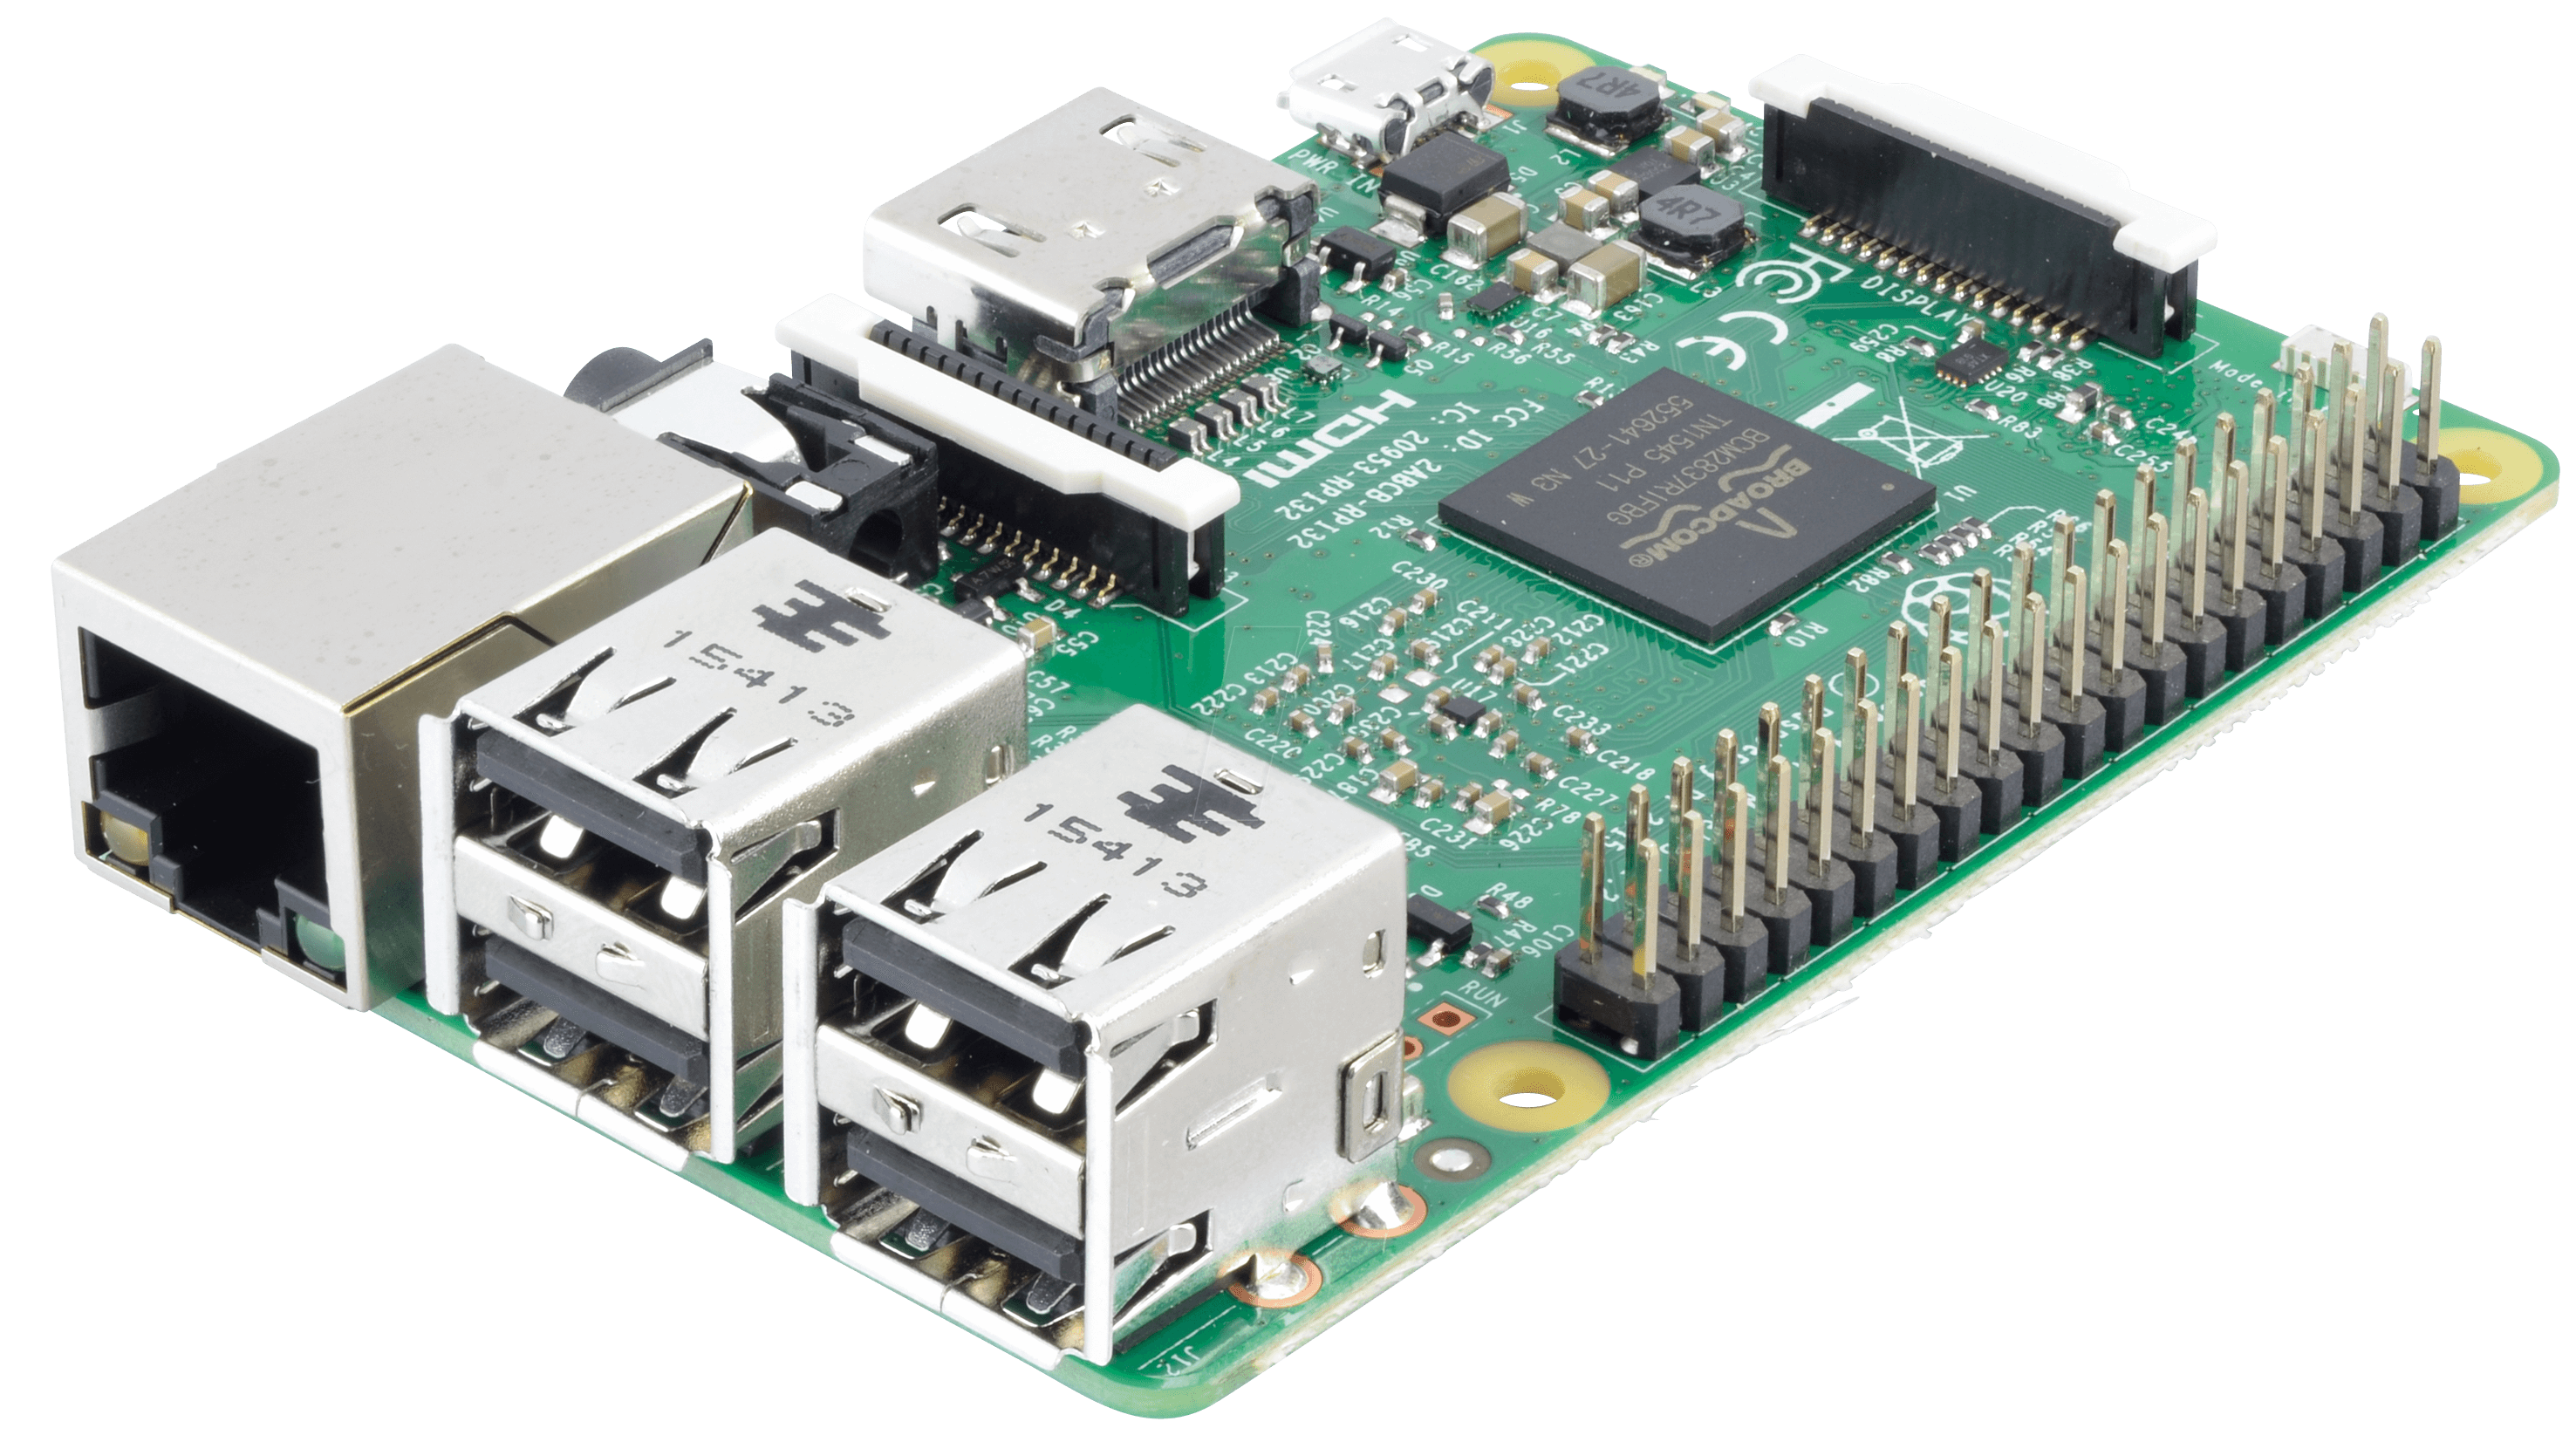
\includegraphics[width=\linewidth]{gfx/RPi3}
	
	Raspberry Pi 3
} Another familiar environment, powerful enough to debug and hold the delegated \ac{P2ABCE} Java services (User, Verifier, \dots) of P2ABC with its 1GB of RAM, and with two network interfaces it's perfect to work as the gateway for the IoT devices to the Internet.

Only a microSD with enough space to burn the binary with the OS is needed to plug\&play with the Raspberry Pi. We use Raspbian, a stable Debian based distro, recommended by the Raspberry Pi designers, and ready to use with the \ac{P2ABCE} compiled \textit{.jar} services.

\begin{table}[h]
	\myfloatalign
	\begin{tabularx}{0.75\textwidth}{ll} \toprule
		CPU & ARMv8 64bit quad-core 1.2GHz \\
		RAM & 1GB \\
		Storage & microSD \\
		Firmware & Raspbian (Debian based distro) \\
		Connectivity & Wifi n + Ethernet \\
		Power & 5V 2A \\
		\bottomrule
	\end{tabularx}
	\caption[Raspberry Pi 3 Specifications]{Raspberry Pi 3 Specifications.}
	\label{tab:RPi3Specs}
\end{table}





% C as pure as possible aiming to lower powerful devices without C++ support or std libraries
% LibGMP and OpenSSL for PoC
% CMake for portability and easy to config cross-compilation
% Java for P2ABCE
% Docker for building environments, both maven and LEDE SDK

\subsection{Software}

The development is divided between the \ac{IoT} device code and the \ac{P2ABCE} services.

\hfil

The P2ABCE is already written in Java, and few modifications will be done to the code in comparison to the existing project size, so we will continue using Java with the P2ABCE part.

\hfil

All IoT devices, have a C cross-compiler, some even a C++ cross-compiler. The worst case scenario is that one must write assembly code, and that code will be specific of that target, so we won't consider them.
If now we focus on the most constrained devices, we could find out that some can't compile C++, some may not have many common libraries, and that the memory limitations they face make practically impossible to use dynamic memory, if we want to avoid very possible execution malfunctions.

For that reason, the developed code for IoT devices must be written with standard C without using dynamic memory.

\hfil

A project with thousands of lines of code can't be written in a single file. And to manage the compilation of multiple files, organized in various directories, we will use CMake.

CMake has many advantages over Makefiles:

\begin{itemize}
	\item Cross-platform. It works in many systems, and more specifically, in Linux it generates Makefiles.
	\item Simpler syntax. Adding a library, files to compile, set definitions, etc. can be done with one CMake command, with rich documentation on the project's \href{https://cmake.org/cmake/help/latest/}{website}.
	\item Cross-compilation. With only a \href{http://www.vtk.org/Wiki/CMake_Cross_Compiling#The_toolchain_file}{\small{CMAKE TOOLCHAIN}} file, CMake sets up automatically the cross-compilation with Makefiles and the C/C++ cross-compiler provided.
\end{itemize}


\hfil

Although the ideal final code is pure C without external libraries or dynamic memory, the \ac{PoC} uses three major libraries:

\begin{itemize}
	\item OpenSSL: Provides reliable and tested AES and SHA256 implementations.
	\item LibGMP: Provides multiprecision integer modular arithmetic.
	\item cJSON: Provides a JSON parser to store and read the status in a human readable way.
\end{itemize}

These three libraries are used to implement different interfaces in the project, and C implementations of these interfaces should replace the external libraries in the future.

\hfil

Finally, we use Docker to deploy the compilation environments:

\paragraph{P2ABCE environment} A container with OpenJDK 7 and Maven installed, with the Idemix maven plugins installed following the project \href{https://github.com/p2abcengine/p2abcengine/wiki/How-to-Build-the-ABC-Engine}{instructions} to use Idemix as the Engine for P2ABCE.

\paragraph{LEDE SDK environment} A container with CMake and the LEDE SDK \citep{ledeproject} installed and configured for the Omega2 target.

The Dockerfiles can be found in the Appendix.
%TODO